\chapter{Local Remote Procedure Call}
\section{Introduction}
% give a short introduction into the problem, the goal, the approach,
For intra-core communication, our OS builds on top of the already provided Lightweight Message Passing (LMP).
Our communication is done via a framework we have built on top of bare LMP channels.
It is part of a wider abstraction of our general remote message passing (RPC) framework,
which works by combining LMP and inter-core communication, which is achieved using user message passing (UMP).

The resulting RPC framework abstracts those two frameworks under a single message passing interface
for any process on any core. In this chapter, we only talk about LMP. Any mention of RPC
in this chapter concerns only the abstraction of LMP in our codebase.

\section{Where is it used}
We use LMP channels for every newly spawned child process. Every process creates 
establishes one LMP channel to the memory server, one for the init-server (which handles e.g. spawn requests),
and one to the serial driver. Later one, we will see that our nameserver, which allows the registration of 
services also uses LMP for communication to clients.

\section{Designing The Message Passing Infrastructure}
% Use cases: memory, init-comm, serial driver, between processes
% Either async vs sync -> easily usable for a server as well as for a client
% Choices: All using same channel. Locking -> where is concurrency possible
%          Separate channels for separate uses; also: how is state passed in messages
Lightweight Message Passing (LMP), which is used to communicate between processes
on the same core is merely a means of communication. On top of such a functionality,
various designs can be implemented for allowing a safe, reliable and usable system
for communication. We will see in this chapter how we've built a system which allows
an easy integration for use in a Memory Server (to distribute RAM capabilities 
to processes), a Serial Server (for input/output to a screen) as well as an Init Server 
(for communication to the \texttt{init} process).

Of interest are the different choices one could use LMP to communicate asynchronously and/or 
synchronously. Also, it's of big interest to utilize the asynchronous nature of LMP to
achieve high concurrency during operation. Lastly, while a functioning protocol for the basic
functionalities required (communication with init, memory and serial servers) 
should surely be logically separated, there are many options how one might separate them physically.
These can be isolated components over different channels, or handled by a single channel all-together.

\subsection{Blocking vs Non-Blocking}
To embrace the non-blocking nature of LMP achieved through upcalls, we provide an 
easy interface for a process to register for the reception of such messages. This interface is 
access through the function 
\begin{minted}{c}
errval_t aos_lmp_register_recv(struct aos_lmp *lmp, process_msg_func_t process_msg_func);
\end{minted}
which is defined in \texttt{aos/aos\_lmp.c} for registering a server.

\subsubsection{Non-Blocking}
For non-blocking communication, we focused mostly on the use-case of arbitrary servers, 
which offers services to be received and processed in an endless-loop.

Since any server (e.g. the memory server) can register such a handler, it becomes trivial to 
implement servers. If registered through the interface, the framework automatically takes care of 
re-registering the process function after the reception of any request. 
The only responsibility we give to the server is then to actively wait for 
messages to come in, which can be done in the all-too-familiar manner:

\begin{minted}{c}
    while (true) {
        err = event_dispatch(default_ws);
        if (err_is_fail(err)) {
            // handle error
        }
    }
\end{minted}

\subsubsection{Blocking}
When talking about blocking communication, we have mostly client-applications in mind. 
While a server usually only responds, a client requests.

In our cases throughout the course, these requests of clients made sense to be blocking, 
so that user-code only continues to run after a response has been received.

Our approach to implementing blocking LMP has been one of the greatest downfall in
our operating system and has been proven to be very much against the idea of the strengths of LMP.

Blocking communication is achieved by polling on the channel until a message has been received.
As stated, having send-then-receive patterns in mind, we provide a call for doing 
both at once:

\begin{minted}{c}
errval_t aos_lmp_call(struct aos_lmp *lmp, struct aos_lmp_msg *msg);
\end{minted}

Using this interface, a client can send a request inside
\begin{minted}{c}
    struct aos_lmp_msg *msg
\end{minted}
and then await the response, which is stored in a field of the \texttt{lmp} struct above.

The question that the reader familiar with the LMP infrastructure of Barrelfish might ask is
why we decided to poll on messages for receiving responses on client requests.
In an older design, we implemented blocking communication through receiving the message asynchronously 
by registering a receive handler and just waiting for a response using \texttt{event\_dispatch()} again.
However, due to race conditions between different client calls, we abandoned this idea for the time being. 
While the polling worked as a temporary solution, we never got to the point where a rewriting of the client receiving
logic was possible, especially since the integration of our individual projects led to many critical bugs of higher priority.

Further, we only fully understood stack-ripping and methods to call manually stack-managed code
into automatically stack managed code one week before the deadline. It was only at that time that
we also learned about polled waitsets.

We're still convinced that this improvement would lead to a performance increase in 
our implementation, especially under heavy load.

\section{Binding}
Before using a channel, it needs to be created. 
In our case, we needed to create channels between the \texttt{init} process and a newly-spawned
child process. After the channel has been established between the two parties, 
it can be used for communication. During the implementation, we were very confused by the notion of
endpoints, waitsets and what a channel actually embodies. The book alone did not help
us understand the structure and process well enough. Through a lot of trial and error,
we later successfully managed a first request.
In the following, we describe how channels are established.


Let's have a look at the init server.
When a new child process is spawned, the \texttt{init} process hands it an endpoint-capability
to itself. That way, the child already knows which channel it needs to bind to. 
Given that capability, the child has enough information to contact \texttt{init}, and 
\texttt{init} has enough information to receive messages. To also allow \texttt{init}
to send to the child, the child process will create a new endpoint and send it to \texttt{init}
in a binding handshake. Using this endpoint, both parties can then send and receive.
At this point, the channel has been fully established.


\section{RPC State}
During operation, we support sending messages of dynamic size.
Supporting the option to send messages without causing page faults was crucial 
to us. Besides increased performance, it is also necessary for being able to use our memory server.
During page fault, we might need to receive additional memory. However, we are not allowed to cause another
nested page fault in that. For that reason, we added a static buffer to each RPC channel of 4096 bytes, 
which is used to send statically sized RPC messages that fit into it.
That way, functionality like sending RAM over RPC can use an already-mapped memory region for 
receiving messages, thus avoiding page faults. In general, any established 
RPC channel consists of the following components:

\begin{itemize}
    \item A buffer allocated at spawn time for receiving messages smaller than a page, which guarantees
    communication without causing page faults
    \item Knowledge for each message a channel is receiving indicating whether we may allocate a large
    buffer for receiving messages larger than one page, i.e. we may incur page faults using this channel.
\end{itemize}

We now describe the state which is kept by our RPC communication protocol.

\subsection{Message Sizes}
We support sending messages of dynamic sizes. To achieve this, we considered 
either shared memory or breaking messages into smaller packets.
While shared pages will decrease the overall LMP-traffic, we would also 
require additional logic for sharing the pages necessary as well as 
copying a potentially large source buffer to this large memory region.

Many questions arise:
\begin{itemize}
    \item Who has read/write access to the shared page? 
    \item When is this shared page unmapped?
    \item At which size of payload will shared memory make sense?
\end{itemize}
On the receiving side, the data would need to be copied out of the shared region 
into newly allocated memory. The copying is necessary since the sender 
might want to unmap the shared memory region at some point and it shouldn't be 
the case that both processes modify the same shared memory region.

Splitting messages into multiple parts has a very straight-forward structure 
without having the additional bookkeeping complexity shared pages have.


In the end, we decided to use the message-splitting approach.
More precisely, any message packet we send over LMP is sized at most 32 bytes
large. This block size was chosen arbitrary and it would have been interesting to measure
to compare performance with larger block sizes.

\subsection{Message Structure}
Below, we describe the structure of a whole message of dynamic size.
\begin{minted}{c}
struct aos_rpc_msg {
    aos_rpc_msg_type_t type;
    char *payload;
    size_t bytes;
    struct capref cap;
};
\end{minted}
Every message sent over an LMP channel contains a message type determining 
the type of request, the actual payload, payload size and optionally, 
also a capability to be transferred through the channel. 
Additionally, to the beginning of a message to be sent, we prepend its size 
to the payload. That way, the receiving size can determine the size of an 
incoming message and knows how many more are to be expected.

\subsection{Invariants}
To achieve thread-safety, our LMP communication protocol 
follows the following invariants:
\begin{itemize}
    \item Client send-receive patterns are atomic with respect to the channel
    \item Server receive-send patterns are atomic with respect to the channel
    \item No process uses a channel as a server and client at the same time
\end{itemize}
These invariants allow us to avoid race conditions and the guarantee that 
when a client receives a response, it will be the response to the client's
request and not the response to any other request from another thread.
To achieve that, it's also necessary that no process uses a both server and client at the same time.
With that at hand, we have a total order of RPC requests of a client and no 
response-mixups, where a client receives a response which is meant for another thread using the same channel.

Note at last that these invariants are only concerning a single channel.
Different channels follow no requirements with respect to other channels 
and can be treated separately.

\section{Implementing Functionality on Top of LMP}
Now that the structure of our use of LMP-channels have been explained, 
lets have a look at how they are used to build actual services and how 
they interleave at the example of our memory, terminal and init servers.

\subsection{Physical Separation of Services}
By our invariants, send-receive and receive-send  patterns must be atomic. Thus, we can't allow an RPC call to 
start recursive RPC calls (which would be breaking atomicity). Since dynamically-sized messages 
need to allocate dynamic memory when receiving an arbitrary-sized response, 
it could otherwise happen that memory is requested during an RPC call.
This could (and did) lead to recursive page faults and other unexpected behaviour.
Further, a channel that is registered a waitset cannot at the same time be
used for blocking calls as the received message will also result in an upcall.

Therefore, each process gets two different channels to the core-local init process:
one to register in the waitset to receive requests from init (the server channel) and
one to send (blocking) requests to init (the client channel). Further, we decided
to establish a separate memory channel with flags such that it will never
enter a code path incurring a page fault.

Of all these channels only the server channel is registered with the default
waitset as the other channels are only used in a blocking manner.

\subsection{Memory Server}
The memory server runs on the \texttt{init} process and receives RAM cap requests.
Since these requests and responses are all statically sized, no recursive page faults 
happen. Since our interface allows sending/receiving capabilities, this 
is already enough to implement the memory server.
Similar to the \texttt{init} server, it performs a handshake with the child process
when it is spawned. 
\subsection{Terminal Server}
The terminal server runs on its own channel and communicates with the UART driver, which will be explained in the Shell chapter.
\subsection{Init Server}
% TODO
The init server registers the following handle-function 
\begin{minted}{c}
    errval_t init_process_msg(struct aos_lmp *lmp)
\end{minted}
It is responsible for handling spawn-requests, sent strings/numbers, PID lookups to receive 
the name of a process given its PID, and clients can also request to receive a list of all PIDs.

All requests to this service are stateless - all information for a request must be 
contained in the request itself.


\section{Encountered Problems}
We had a few problems with our initial RPC implementation, 
which after some revisions led to the invariants stated above. Some of these problems were:
\begin{enumerate}
    \item Mixing server and client functionality led to race conditions.

    \item When implementing support for page faults, we realized that it must be possible 
to guarantee that a RPC call will cause no recursive page fault.

    \item When mixing LRPC with URPC, it has become crucial to abstract LMP and UMP as much 
as possible, to avoid a confusing interface for a programmer in user-space.
\end{enumerate}

\section{Transfer Speed}
We plotted the transfer speed of our LMP channel for different string sizes by using \texttt{aos\_rpc\_get\_string}
and measuring the total time.
\begin{figure}
    \centering
    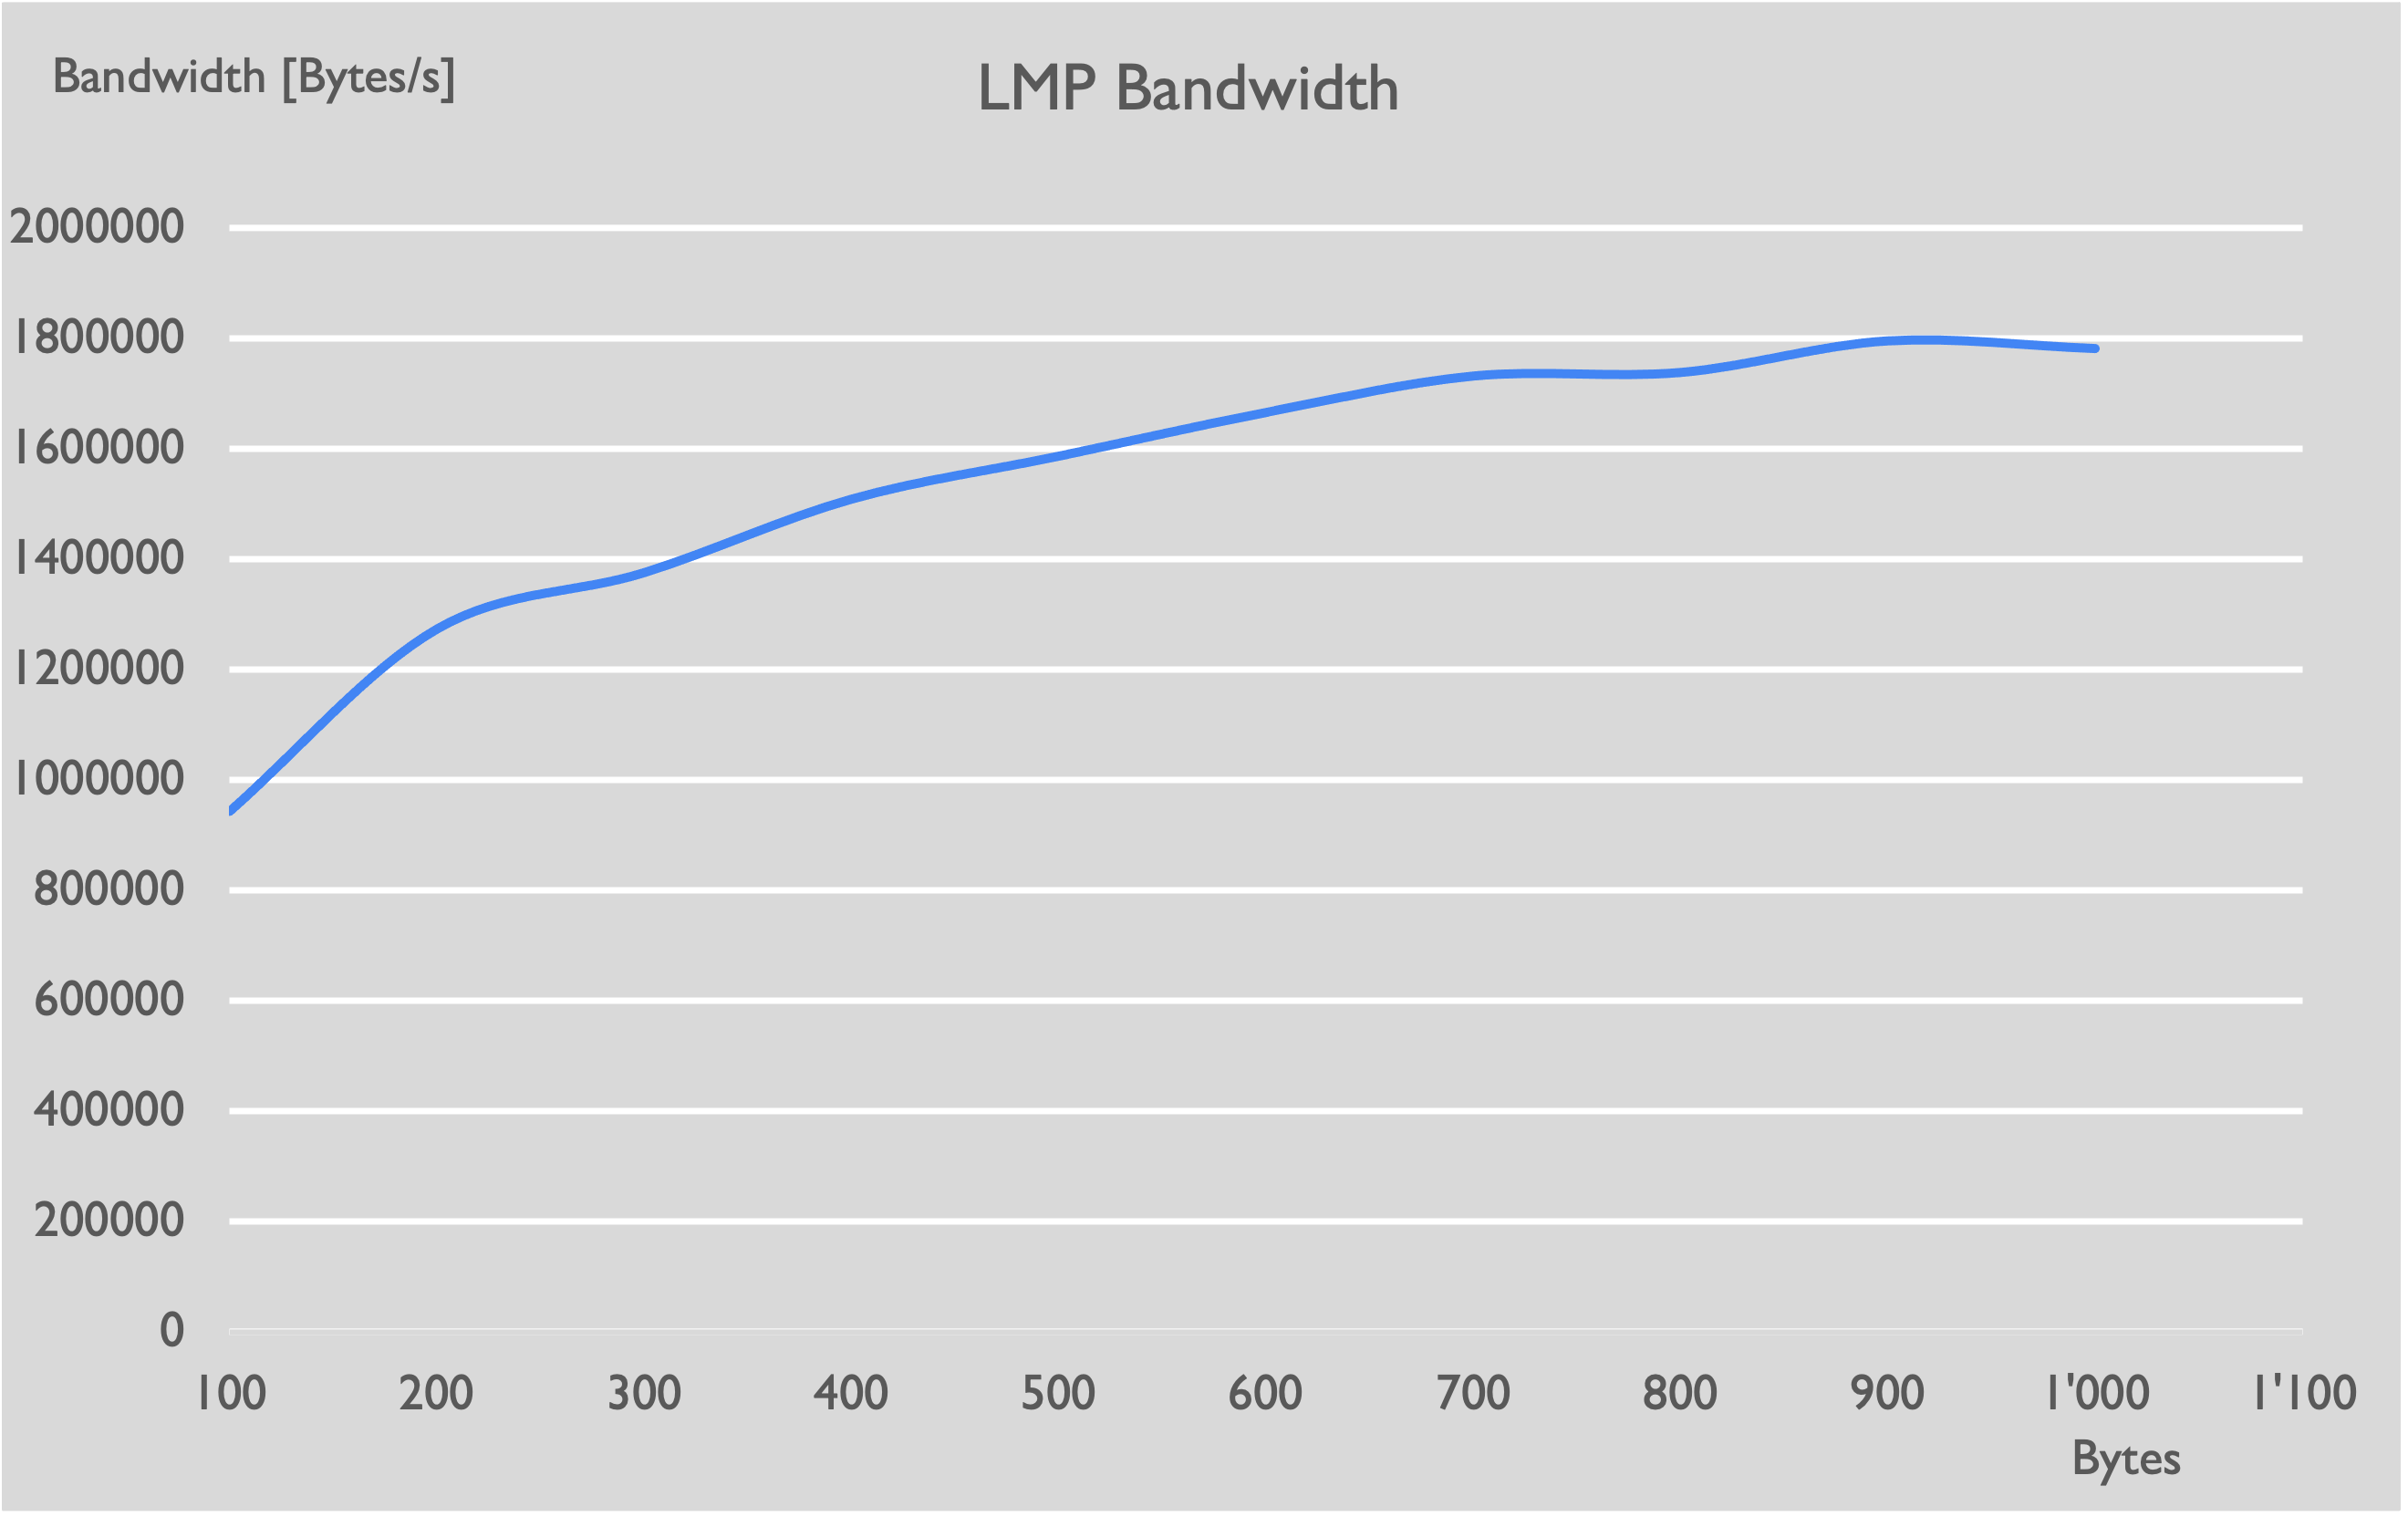
\includegraphics[scale=0.7]{lmp_bandwidth.png}
    \caption{LMP Bandwidth}
    \label{fig:my_label}
\end{figure}
As we can see, we reach transfer speeds of up to 1.8GB/s, which is roughly 10 times lower than the usual DDR3. The overhead of the first message which needs to be received can be seen by the lower bandwidth for smaller sizes, however the performance soon is saturated.

\section{Analysis} % Problems; performance; hindsight
Given more time, we would be interested to play with different packet sizes. As stated,
we currently use packets of 32 bytes. Benchmarking performance with other sizes 
would be a good idea. However, we weren't too concerned with this, since most of the RPC
messages we send (and crucially, the ones which are sent most frequently) fit into a single packet.

Another improvement would be to look at rewriting blocking reception of RPC messages,
which currently uses polling to check if an incoming message exists. As said, we 
abandoned the idea of using upcalls for receiving responses to blocking client requests due to race conditions 
which resulted from failure to abide by our stated invariants. Given more time, 
this would be a good performance optimization and a crucial improvement to our system.

Avoiding the idea of message-splitting altogether, 
using the shared-memory approach for dynamically sized messages could be 
analyzed further and performance compared. We suspect that starting from some size, 
sharing memory will outperform message-splitting substantially.


% extra:
% big messages